% http://wiki.eclipse.org/Development_Resources/HOWTO/Bugzilla_Use
%   The severity tags aren't used much, except to distinguish enhancements from bugs. Typically the users specify severities as they see fit.


% http://wiki.eclipse.org/Bug_Reporting_FAQ
%   when a test pass comes up a component owner can build a query that searched for resolved bugs
%   After testing that the fix worked a resolved bug can be transitioned to verified, directly to closed, or in fact, reopened. 
%   By searching for bugs with a Status of verified and a resolution of fixed developers can come up with release notes.
%   Severity is assigned by a user and describes the level of impact the bug is having on them. Priority is assigned by the developer and describes the importance a developer places on fixing the bug.

\begin{section}{Introduction}

Bug repositories (or bug tracking systems) have for a long time been used in software projects to support coordination among stakeholders. Such systems record discussion and progress of software evolution activities, such as corrective, perfective, and ... changes \cite{Antoniol2008}. Hence, bug repositories are an opportunity to researchers who intend to investigate issues related to the quality of the product and of the process of software development team.
%, or even issues regarding the nature of software development itself.

The information contained in bug repositories has been used in order to predict fault-proneness, to unveil developers' roles from data, to characterize transfer of work in software projects, and so on. Also, it has been used to investigate beliefs in software engineering related to software quality, such as the impact of developer turnover and of collective ownership on the occurrence of bugs.

However, mining bug repositories has its own risks. Previous research has identified problems of missing data (e.g., rationale, traceability links between reported bug fixes and source code changes) and inaccurate data (e.g., misclassification of bugs) \cite{Aranda2009,Bird2009,Nguyen2010,Ayari2007}.

  In previous research [cite report], we tried to assess the impact of independent verification of bug fixes on software quality, by mining data from bug repositories. 
  We relied on reported verifications tasks, as recorded in bug reports, and interpreted the recorded data according to the documentation for the specific bug tracking system used.
  As the partial results suggested that verification has no impact on software quality, we questioned the accuracy of the data about verification of bug fixes, ad thus decided to investigate how verification is actually performed and reported on specific software projects.
	
	In particular, we are interested in answer the following exploratory research questions for a limited set of projects:

	\begin{itemize}
		\item \textbf{How} is the verification performed: are there performed ad hoc tests, automated tests, code inspection?
		\item \textbf{Who} performs the verification: is there a dedicated team for QA? 
		\item \textbf{When} is the verification performed: is it performed just after the fix, or is there a verification phase?
		% \item How is the distribution of verification across developers?
		% \item Is there a dedicated team for QA?
	\end{itemize}

	
% \TODO why the VERIFIED status is so important?

% In summary, for researchers who intend to use data from bug tracking systems, it is not sufficient to understand the data fields in a bug report the way they are documented in the system's documentation. The research should also investigate whether the data fields are used often, whether they are used accordingly to the documentation, and even if the data fields are used consistently across the developers.

% In this paper, we investigate the status of a bug, a data field present in most bug tracking systems that reports the progress of the bug solving activity. In particular, we focus on the activity of verification of a fix. We are interested in answering the following exploratory research questions:

% For research question xx, qualitative of a small sample. 
% For research question xx, all bugs were considered.

\end{section}

\begin{section}{Background}
% Bug workflow. Bugzilla. \cite{Bird2009}

% Reposit ́orios de bugs. Arquivam relat ́orios de defeitos e solicitac ̧ ̃oes de mudan ̧ca. Tais reposito ́rios ajudam os desenvolvedores a registrar, discutir e acompanhar a situa ̧ca ̃o de cada solicita ̧c ̃ao, desde a atribui ̧ca ̃o de uma solicita ̧ca ̃o a um desenvolvedor at ́e a verifica ̧c ̃ao da corre ̧c ̃ao ou melhoria. Exemplos incluem o Bugzilla, o Trac e o Jira.

Bug tracking systems allow users and developers of a software project to manage a list of bugs for the project. Usually, users and developers can report bugs, along with information such as steps to reproduce the bug, its severity and the operating system used. Developers choose bugs to fix and can report on the progress of the bug fixing activities, ask for clarification, discuss causes for the bug etc.

In this research, we focus on Bugzilla, an open source bug tracking system used by notable software projects such as Eclipse, Mozilla, Linux Kernel, Open Office, Apache, and companies such as NASA and Facebook\footnote{Complete list available at http://www.bugzilla.org/installation-list/.}. The general concepts from Bugzilla should apply to most other bug tracking systems.

One important feature of a bug that is recorded on bug tracking systems is its status. The status records the progress of the bug fixing activity, and, as such, provides data to software engineering studies. Figure \ref{fig:bugzilla} shows each status that can be recorded in Bugzilla, along with typical transitions between status values, i.e., the workflow.

\begin{figure}[ht]
	\centering
		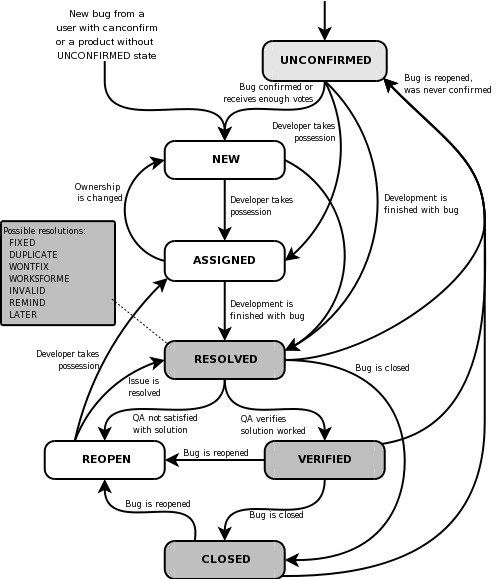
\includegraphics[scale=0.4]{bugzilla.png}
	\caption{Workflow for Bugzilla. Source: \url{http://www.bugzilla.org/docs/2.18/html/lifecycle.html}.}
	\label{fig:bugzilla}
\end{figure}

In the simplest cases, a bug is created and receive the status \texttt{UNCONFIRMED} (if it was created by a regular user) or \texttt{NEW} (if it was created by a developer). Next, it is ASSIGNED to a developer, and then it is RESOLVED, possibly by fixing it with a patch on the source code. The solution is then VERIFIED by someone in the quality assurance team. If it passes the quality requirements, it is CLOSED when the next release of the software is released. If it does not pass the quality requirements or if the solution only partially fixes the problem, the bug is REOPENed.

\TODO Roles: reporter, fixer, verifier, reopener, closer.

In order to understand the bug fixing process of a software team, however, it should be possible to know what activities are performed upon change of status. For example, what steps are made before changing the status of a bug to RESOLVED (FIXED)? Is the patch applied to the version control system? Is it presented as diff file attached to the bug report? Is there a build available to end users containing the patch (e.g., a nightly build)? The documentation for Bugzilla does not prescribe specific activities for marking a bug as RESOLVED, relegating instead this decision to each software project.

Similarly, what do developers do before marking a bug as VERIFIED? Bugzilla documentation states that, when a bug is VERIFIED, it means that ``QA [quality assurance team] has looked at the bug and the resolution and agrees that the appropriate resolution has been taken''\footnote{\url{https://landfill.bugzilla.org/bugzilla-3.6-branch/page.cgi?id=fields.html}}. Again, the definition is broad, although it assumes the existence of a QA team.

The developer documentation for both Eclipse and NetBeans are unclear about how the verification of a bug fix is performed. So, what forms of  software verification are they used in the verification process of these projects?
% In some parts they mention running unit tests, and running a patched version of the software and try to reproduce the bug.

Software verification techniques are classified in static and dynamic [cite Sommervile]. Static techniques include source code inspection, automated static analysis, and formal verification. Dynamic techniques, or testing, involve executing the software system under certain conditions and comparing its actual behavior with the intended behavior. Testing can be done in an improvised way (ad hoc testing), or can be compiled in a list of test cases, which can then be automated (e.g., as unit tests).

While mining bug repositories, one cannot assume that the VERIFIED status comprises all forms of software verification. Also, one cannot rely on the information provided by the bug tracking system or the developer documentation for a project, since it can be too generic to be useful. Such information can only be assessed by taking a close look on actual bug reports.

% O bug não se manifesta após a aplicação da solução.
% A solução não gera novos bugs.
% O código da solução segue as convenções de codificação e políticas do projeto.
% A solução possui uma boa relação custo-benefício — isto é, ou não existem soluções melhores ou a solução é um paliativo por conta da alta complexidade de uma solução melhor.
% 
% Minha expectativa, portanto, é que, antes de o bug ser marcado como VERIFICADO, ele passe pelas seguintes atividades:
% 
% Aplicação do patch com a solução do bug na versão do software onde o bug foi encontrado.
% Execução do software com o bug, seguindo os passos para reprodução do bug, e verificando que o bug não se manifesta
% Inspeção do código-fonte. Deve ser verificada a aderência às convenções de codificação do projeto e a outras políticas (por exemplo, cada patch deve vir com testes de unidade).
% Execução de testes de unidade (se houver). Deve se verificar que todos os testes passam.

\end{section}

\begin{section}{Method}

	% \item How is the verification actually performed?
	% \item When is the verification performed (i.e., just after the fix, or is there a specific period for the verification of fixed bugs?)
	% \item Who performs the verification?

In order to answer our exploratory research questions, we followed the following method:

\begin{enumerate}
	\item \textbf{Data extraction}: we have obtained publicly available raw data from the Bugzilla repositories of two popular integrated development environments, Eclipse and Bugzilla.
	
	\item \textbf{Data sampling}: we have chosen two subprojects. After that, we sampled bugs with interesting characteristics.
	
	\item \textbf{Data analysis}: we have read the full bug reported for the sampled bugs. Also, we have performed quantitative analysis on all bugs.
	
	\item ...
\end{enumerate}

\begin{subsection}{Available Data}
	
	In order to perform the desired analysis, we needed access to all data recorded by Bugzilla for a specific project. We have found such data for two projects---Eclipse and NetBeans---from the domain of integrated development environments. The data were made available as part of the Mining Software Repositories 2011 Challenge\footnote{\url{http://www.msrconf.org/msr-challenge.html}} in the form of MySQL database dumps. The files contain all tables from the respective databases, except for the tables containing information about developers.
	
	% We have had access to Eclipse Bugzilla database from October, 2001 to June, 2010, and to NetBeans Bugzilla database from ... to .... The data was made available as part of the Mining Software Repositories 2011 Challenge\footnote{\url{http://www.msrconf.org/msr-challenge.html}} as a SQL dump. The SQL dump contains all information recorded by Bugzilla for the projects (except for information about developers, which was removed for privacy reasons).

	Eclipse development began in late 1998 with IBM\footnote{\url{http://www.ibm.com/developerworks/rational/library/nov05/cernosek/}}. It was licensed as open source in November, 2001. In 2004, IBM created the Eclipse Foundation in order to reduce the perception of Eclipse as a IBM-controlled project.
	
	NetBeans\footnote{\url{http://netbeans.org/about/history.html}} started  as a student project in 1996. It was bought by Sun Microsystems in October, 1999, and it was open sourced in March, 2000.

	Both Eclipse and NetBeans are composed of many subprojects. The data comprises all bug reports from all Eclipse subprojects from October, 2001 to June, 2010, and from all NetBeans subprojects from June, 1998 to June, 2010.
	
	There are 316,911 bug reports for 155 subprojects in Eclipse, and 185,578 bug reports for 39 subprojects in NetBeans.
	
\end{subsection}

\begin{subsection}{Sampling of Bug Reports}
	
	In order to obtain insight about the research questions, we read a sample of bug reports from both projects. For each project, two subprojects were chosen randomly among the projects with most verified bugs, resulting in the following subprojects: Eclipse/Platform, Eclipse/EMF, Netbeans/profiler, Netbeans/versioncontrol. We have sampled 20 bug reports for each subproject, totalizing 80 bug reports.
	
	\TODO this sampling was made just for the preliminary, qualitative analysis. Maybe we should describe preliminary analysis as an unstructured inquiry (instead of detailing the methods for it).
	
\end{subsection}

\end{section}

\begin{section}{Results and Discussion}
	
\begin{subsection}{Preliminary Analysis}
	Some insights were gained in this step, partially answering the who, when, and how questions:
	
	\begin{itemize}
		\item [how] In some projects, the status VERIFIED does not correspond to software verification. In Eclipse/EMF, for example, it means that the fix is available in a build that is promoted on the project website\footnote{\url{http://wiki.eclipse.org/Modeling_PMC_Meeting,_2007-10-16}}.
		\item [(who)] In the NetBeans subprojects that were analyzed, it was common that the reporter also verified the fix. In some bugs, this was necessary since the developer was not able to reproduce the bug.
		\item [(who, when)] Often, the fixer verifies the bug just after marking it as fixed.
		\item [(when)] Sometimes, several old bugs are marked as VERIFIED at the same time.
		\item [(how?)] In Eclipse/Platform, it is common that the fixer requests someone else to verify the fix (``Please verify, Tom'').
		\item [(how)] In Eclipse/EMF, bug #249436, one developer rewrites the patch submitted by other developer.
		\item [(how)] In Eclipse/EMF, bug #269789, a test case is used to assess the proposed fix.
	\end{itemize}
\end{subsection}	
	
\begin{subsection}{RQ1: How Are Bugs Verified?}
	
	We analyzed cases in which the bug is fixed, the fixer asks someone else to verify the fix, and then the bug is reopened.

	Findings: ...
	
\end{subsection}

\begin{subsection}{RQ2: When Are Bugs Verified?}
	
\end{subsection}

\begin{subsection}{RQ3: Who Verifies Bugs?}
	
	We counted the number of times each developer verified or fixed a bug. We consider that, if a developer is primarily concerned with quality assurance, then s/he verifies much more bugs that s/he fixes.
	
	We defined ratio as ...
	
	The verified/fixed ratio for the four projects is shown on Table XXX.
	
\begin{verbatim}
*** eclipse-platform 
Verifiers: 4(2.38095238095238%) = 1.08523937083591% of verifications
Fixers: 30 -- 17.8571428571429%
Total developers: 168 

*** eclipse-emf 
Verifiers: 0(0%) = 0% of verifications
Fixers: 4 -- 30.7692307692308%
Total developers: 13 

*** netbeans-profiler 
Verifiers: 3(21.4285714285714%) = 89.9688958009331% of verifications
Fixers: 2 -- 14.2857142857143%
Total developers: 14 

*** netbeans-versioncontrol 
Verifiers: 5(20.8333333333333%) = 93.2291666666667% of verifications
Fixers: 6 -- 25%
Total developers: 24
\end{verbatim}
	
	In NetBeans it is possible to infer the existence of a QA team, composed by approximately 20\% of the developers, that performs about 90\% of all verifications.
	
	In the Eclipse subprojects, there is no evidence of a dedicated QA team. In Eclipse/EMF no developer focus specifically on verification (it should be remembered that verification in EMF has a peculiar meaning). In Eclipse/Platform, only 2\% of the developers focus on verification tasks, however, they contribute only to 1\% of the verifications.
	
\end{subsection}

\end{section}

\begin{section}{Conclusion}
  The VERIFIED status is used in a variety of distinct ways, not always consistent with the traditional definition of software verification ...
	
	With the knowledge obtained from this exploratory research, we can improve and extend our previous work on the impact of independent verification on software quality. Examples of refined questions:
	
	\begin{itemize}
		\item Does independent verification improve software quality when it is performed by developers from the QA team?
		\item Does independent verification improve software quality when it is performed as an separate phase of the software release cycle?
		\item Does independent verification improve software quality when a particular verification technique (e.g., inspections, unit testing) is used?
	\end{itemize}
	
\end{section}

\section*{Acknowledgment}

The first author is supported by FAPESB under grant BOL0119/2010.
